\newpage
\section{Training Procedure of Unified Latent-MI Probe}
\label{app:d}

This appendix provides a detailed description of the Unified Latent-MI Probe (ULP) training procedure used to quantify the information content of latent representations, corresponding to the variational upper bound estimation described in Section~\ref{sec:mi_estimation}.

\subsection{Hidden State Extraction}

Given a trained latent CoT model with parameters $\theta$, we extract hidden states from the continuous latent chain. For a given input question $q$ and its corresponding ground-truth reasoning steps $\mathcal{S} = \{S_1, S_2, \ldots, S_K\}$, the model processes the sequence interleaved with latent blocks. For the $t$-th reasoning step $S_t$, the input context is:
\begin{equation}
    x_t = [\ldots, S_{t-1}, \texttt{<|start-latent|>}, \underbrace{L_{t,1}, \ldots, L_{t,N}}_{N \text{ latent tokens}}, \texttt{<|end-latent|>}]
\end{equation}
where $N=6$ is the default number of latent tokens per step. 

During the forward pass, we extract the hidden state $\mathbf{h}_t \in \mathbb{R}^{d}$ from the \textbf{last latent token} $L_{t,N}$ (where $d=768$ for GPT-2 base). This vector $\mathbf{h}_t$ serves as the numerical realization of the latent state $L_t$ discussed in the main text. The extracted pairs $\{(\mathbf{h}_t, S_t)\}$ from all baselines are stored in half-precision format to construct the unified probing dataset.

\subsection{Probe Architecture}

The probe aims to approximate the posterior distribution $q_{\phi}(S_t \mid L_t)$. We employ a \textbf{Reconstruction Probe} consisting of:

\begin{enumerate}
    \item \textbf{Projection Layer}: A linear transformation $f_\text{proj}: \mathbb{R}^d \rightarrow \mathbb{R}^d$ that maps the model's latent space to the probe's embedding space:
    \begin{equation}
        \mathbf{z}_t = \mathbf{W}_\text{proj} \mathbf{h}_t + \mathbf{b}_\text{proj}
    \end{equation}
    where $\mathbf{W}_\text{proj}$ is initialized from $\mathcal{N}(0, 0.02^2)$ and $\mathbf{b}_\text{proj} = \mathbf{0}$.
    
    \item \textbf{Conditional Decoder}: A pre-trained GPT-2 language model that generates the explicit tokens of step $S_t$ autoregressively. It utilizes a shared embedding table $\mathbf{E} \in \mathbb{R}^{|V| \times d}$.
\end{enumerate}

\subsection{Training Procedure}

To condition the generation on the latent state, we employ a teacher-forcing strategy. The projected latent vector $\mathbf{z}_t$ is prepended to the embeddings of the target reasoning step $S_t = [w_1, w_2, \ldots, w_M]$. The input embeddings passed to the probe decoder are:
\begin{equation}
    \text{Input} = [\mathbf{z}_t; \mathbf{E}[w_1]; \mathbf{E}[w_2]; \ldots; \mathbf{E}[w_{M-1}]]
\end{equation}
This architecture forces the decoder to rely on $\mathbf{z}_t$ for semantic guidance. We first define the per-sample reconstruction loss:
\begin{equation}
    \ell(\mathbf{h}_t, S_t) = -\frac{1}{|S_t|} \sum_{j=1}^{|S_t|} \log P_\phi(w_j \mid \mathbf{z}_t, w_{<j})
\end{equation}
The probe parameters $\phi$ are then optimized to minimize the expected loss over the unified dataset $\mathcal{D}$:
\begin{equation}
    \mathcal{L}_{\text{Info}} = \frac{1}{|\mathcal{D}|} \sum_{(\mathbf{h}_t, S_t) \in \mathcal{D}} \ell(\mathbf{h}_t, S_t)
\end{equation}

Data from all latent models (OS, PS, GR, GC) are combined into a unified dataset to ensure a fair comparison. Figure~\ref{fig:probe_training} illustrates the training dynamics of the ULP. We observe that PS-GR achieves the fastest convergence and lowest final reconstruction loss, confirming its superior semantic fidelity. In contrast, OS-GC plateaus at a significantly higher loss, reflecting the severe information loss caused by rigid geometric constraints. The detailed training hyperparameters are listed in Table~\ref{tab:probe_hyperparams}.

\begin{figure}[h]
    \centering
    % Left side: Figure (Allocating ~58% width for the plot)
    \begin{minipage}[c]{0.58\textwidth}
        \centering
        \caption{\textbf{Per-Model Probe Loss History.} }
        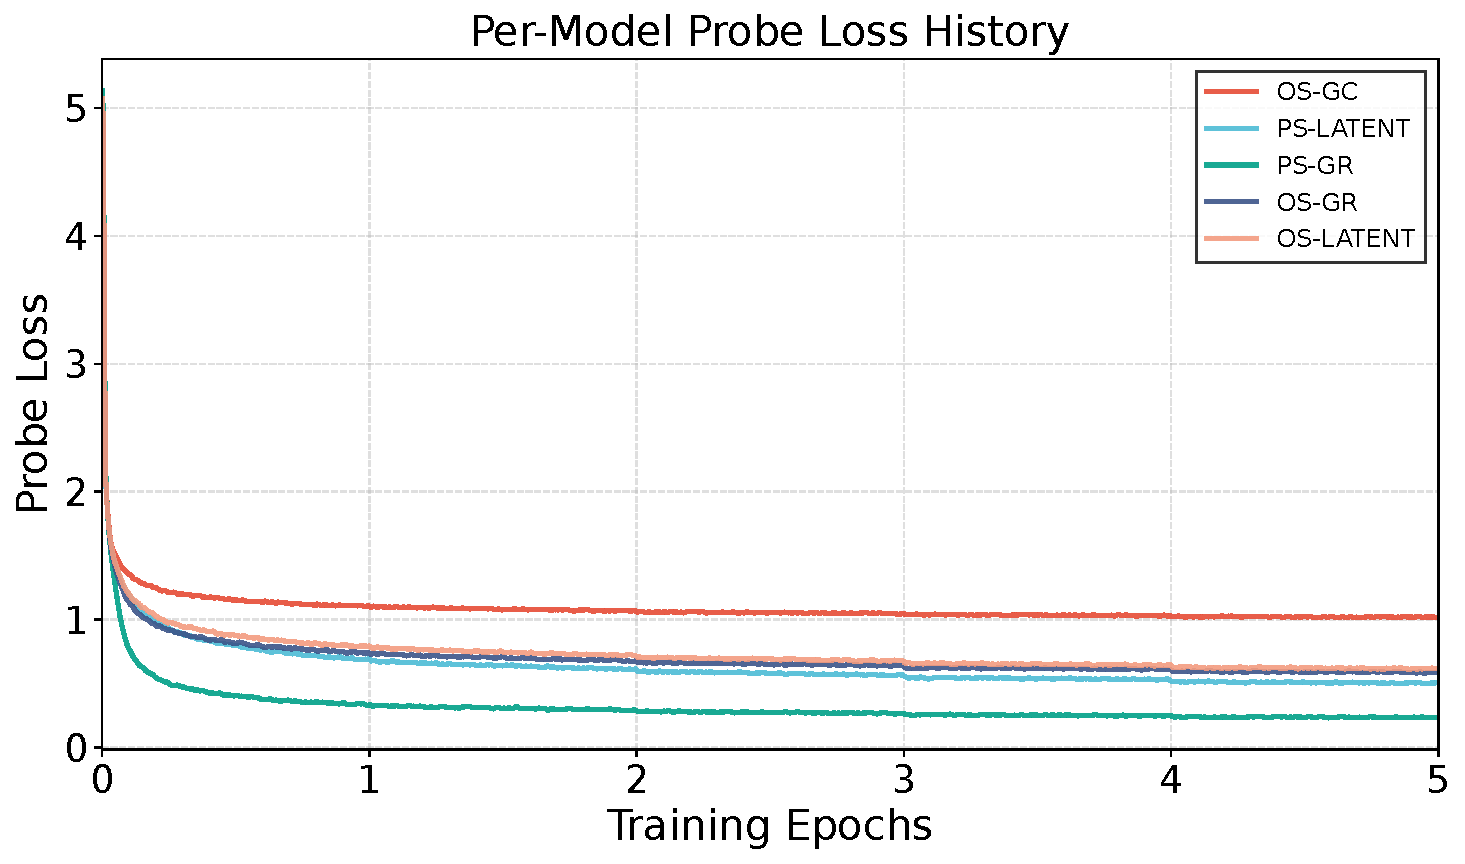
\includegraphics[width=\linewidth]{Figures/App/probe_loss.pdf}
        \label{fig:probe_training}
    \end{minipage}
    \hfill
    % Right side: Table (Allocating ~38% width for the compact table)
    \begin{minipage}[c]{0.38\textwidth}
        \centering
        \captionof{table}{\textbf{Hyperparameters for ULP Training.}}
        \label{tab:probe_hyperparams}
        \small
        \renewcommand{\arraystretch}{1.1} 
        \begin{tabular}{l|l}
            \toprule
            \textbf{Hyperparam} & \textbf{Value} \\
            \midrule
            Optimizer & AdamW \\
            LR & $1 \times 10^{-4}$ \\
            Wt. Decay & 0.01 \\
            Scheduler & Linear (10\%) \\
            Batch Size & 128 \\
            Epochs & 5 \\
            Clip & 1.0 \\
            Precision & FP16 \\
            \bottomrule
        \end{tabular}
    \end{minipage}
\end{figure}

\begin{table}[htb]
\centering
\caption{Probe reliability across architectures. All probes are trained on the same frozen hidden states. Lower values indicate better recovery of explicit reasoning information. }
\label{tab:model_comparison}
\begin{tabular}{lrr}
\toprule
\textbf{Variant} & \textbf{2-Layer MLP} & \textbf{2L-4H Transformer} \\
\midrule
PS-GR      & 1.310 & 0.375 \\
PS-LATENT  & 1.755 & 0.722 \\
OS-GR      & 1.806 & 0.775 \\
OS-LATENT  & 1.861 & 0.824 \\
OS-GC      & 2.145 & 1.049 \\
PS-GC      & 2.194 & 1.097 \\
\bottomrule
\end{tabular}
\end{table}

\subsection{Probe Reliability Across Architectures}
Since recovering an explicit reasoning step from a latent state is naturally a sequence-generation problem, we use a GPT-2 probe as the default decoder-based probe in the main experiments.
To ensure that the observed information hierarchy is not an artifact of this particular probe architecture, we conduct an additional robustness check with three architecturally distinct probes trained on the same frozen hidden states: a two-layer MLP, and a two-layer four-head Transformer. As shown in Table~\ref{tab:model_comparison}, all three probe architectures produce the same ranking over latent representations.


% \subsection{Evaluation Metrics}

% We evaluate the representational fidelity using the mean reconstruction loss on a held-out test set, matching the metrics reported in Figure~\ref{fig:info_hierarchy}:
% \begin{equation}
%     \bar{\mathcal{L}}_{\text{Info}} = \frac{1}{|\mathcal{D}_\text{test}|} \sum_{(\mathbf{h}_t, S_t) \in \mathcal{D}_\text{test}} \ell(\mathbf{h}_t, S_t)
% \end{equation}
% A lower $\bar{\mathcal{L}}_{\text{Info}}$ indicates that the latent state $\mathbf{h}_t$ preserves higher mutual information regarding the explicit reasoning logic $S_t$.